\documentclass[11pt]{article}
\usepackage[english]{babel}
\usepackage{minted}
\usepackage{amsfonts}
\usepackage{amsmath}
\usepackage{amsthm}
\usepackage{graphicx}
\usepackage{subcaption}
\usepackage{booktabs}
\usepackage[left=25mm, top=25mm, bottom=25mm, right=25mm]{geometry}
\usepackage{algorithm}
\usepackage{algpseudocode}
\usepackage[most]{tcolorbox}
\usepackage[colorlinks=true,linkcolor=darkcyan,filecolor=darkcerulean,urlcolor=magenta]{hyperref}

\newtheorem{theorem}{Theorem}[section]
\newtheorem{claim}[theorem]{Claim}
\newtheorem*{question}{Question}

\newtcolorbox{solution}[2][]{breakable,enhanced,adjusted title={#2},colback=codegray,colframe=codegray!50!black}

\linespread{1.0}

\definecolor{codegray}{rgb}{0.98,0.97,0.93}
\definecolor{cottoncandy}{rgb}{1.0, 0.74, 0.85}
\definecolor{darkcerulean}{rgb}{0.03, 0.27, 0.49}
\definecolor{darkcyan}{rgb}{0.0, 0.50, 0.45}

\title{COL351\\Assignment 3}
\author{Mallika Prabhakar (2019CS50440)\\Sayam Sethi (2019CS10399)}
\date{September 2021}

\begin{document}

\maketitle

\tableofcontents

\pagenumbering{arabic}

\newpage
\section{Question 1}

% idea:
% - create dp(i, s1, s2) such that dp(i, s1, s2) is true if we can partition S[1:i] into sets with sums s1, s2, sum(S[1:i]) - (s1 + s2)
% - to find optimal set, iterate over s1, s2 and find min(max(s1, s2, sum(S) - (s1 + s2)))
% - from this value, backtrack to find the optimal partitioning
\begin{solution}{Question 1}\label{ques:1}
    \begin{question}
        Alice, Bob, and Charlie have decided to solve all exercises of the Algorithms Design book by Jon Kleinberg, Éva Tardos. There are a total of $n$ chapters, $[1, \ldots, n]$, and for $i\in [1, n]$, $x_i$ denotes the number of exercises in chapter $i$. It is given that the maximum number of questions in each chapter is bounded by the number of chapters in the book. Your task is to distribute the chapters among Alice, Bob, and Charlie so that each of them gets to solve nearly an equal number
        of questions.\par
        Device a polynomial time algorithm to partition $[1, \ldots, n]$ into three sets $S_1, S_2, S_3$ so that $\max\{\sum_{i\in S_1}{x_i}, \sum_{i\in S_2}{x_i}, \sum_{i\in S_3}{x_i}\}$ is minimized.
    \end{question}
    \tcblower{}
    \begin{proof}[Solution]
        We propose a \textit{Dynamic Programming} solution for this problem. The idea is to generate all possible combinations of $S_1, S_2, S_3$ and then find the best combination of out them. The na\"{\i}ve solution will have an exponential complexity ($O(3^n)$) and hence it needs to be modified so that it can be executed in polynomial time complexity.\\
        We make the following observations to optimise our solution:
        \begin{enumerate}
            \item To find the optimal parititon of $S$, only the sum of each of $S_1, S_2, S_3$ matters
            \item Order of picking elements for each set doesn't affect the solution
            \item Fixing the sum of $S_1$ and $S_2$ uniquely identifies the sum of $S_3$
        \end{enumerate}
        Using these observations we come up with the following DP table:
        \begin{equation}\label{eq:dp_q1}
            \begin{split}
                dp(i, s1, s2) &= dp(i-1, s1-S[i], s2)\vee dp(i-1, s1, s2-S[i])\vee dp(i-1, s1, s2)\\
                &\forall i\in \{1, \ldots, n\}; s1, s2\in\{1, \ldots, sum(S)\}\\
                dp(i, p, q) &= \bot,\ \forall i\in \{1, \ldots, n\}; p, q < 0\\
                dp(0, 0, 0) &= \top
            \end{split}
        \end{equation}
        where $dp(i, s1, s2)$ is $\top$ if we can generate atleast one partition using the first $i$ elements such that any two partitions have sums $s1$ and $s2$
        \begin{claim}
            The dp table generated using the Equation~\ref{eq:dp_q1} is correct, i.e., $dp(i, s1, s2)=\top$ iff there exists a partition using the first $i$ elements with sums $s1, s2, sum(S[1:i])-(s1+s2)$
        \end{claim}
        \begin{proof}
            We will prove the correctness of the claim by induction on $i$.\\
            \textbf{Base case:} $i=0$\\
            $dp(0, s1, s2)$ is $\top$ only when $s1=s2=0$ and $\bot$ otherwise. We know that we can generate only three empty sets using the first $0$ elements and thus their sums will all be $0$. Therefore the base case is true.\\
            \textbf{Induction step:} Assume that the claim is true for $i-1$. Consider $dp(i, s1, s2)$,\\
            The $i\textsuperscript{th}$ element will be present in exactly one of $S_1, S_2, S_3$. Therefore, we have three cases:
            \begin{enumerate}
                \item $S[i]$ is in $S_1$, then the sum of $S_1$ upto the first $i-1$ elements will be $s1-S[i]$ and the sum of the other two sets doesn't change
                \item $S[i]$ is in $S_2$, then the sum of $S_2$ upto the first $i-1$ elements will be $s2-S[i]$ and the sum of the other two sets doesn't change
                \item $S[i]$ is in $S_3$, then the sum of $S_3$ upto the first $i-1$ elements will be $sum(S[1:(i-1)])-(s1+s2)$ and the sum of the other two sets doesn't change
            \end{enumerate}
            Thus, the only possibilities for valid partition sums using the first $i$ elements are exactly those when we can generate atleast one of the above three parititons using the first $i-1$ elements. The transition equation given in Equation~\ref{eq:dp_q1} exactly captures this. We have shown that for $dp(i, s1, s2)$ to be $\top$, atleast one of $dp(i-1, s1-S[i], s2), dp(i-1, s1, s2-S[i]), dp(i-1, s1, s2)$ must be $\top$. From induction, we know that the
            $(i-1)\textsuperscript{th}$ row of the table is true iff there exists a valid parititon. Therefore, if $dp(i, s1, s2)=\top$ then there exists a partition using the first $i$ elements with sums $s1, s2, sum(S[1:i])-(s1+s2)$. ($\implies$)\\

            We still have to prove the converse, i.e., if there exists a partition using the first $i$ elements with sums $s1, s2, sum(S[1:i])-(s1+s2)$, then $dp(i, s1, s2)=\top$.\\
            To prove this, we observe that the $dp$ table considers all possible sums since $s1, s2$ iterate in the range $\{1, \ldots, sum(S)\}$. Therefore, if there exists a valid solution, the $dp$ table considers it and is assigned $\top$. Else it is assigned $\bot$. ($\Longleftarrow$)
        \end{proof}
        Now that we have proved the correctness of Equation~\ref{eq:dp_q1}, we present an algorithm for computing the same:
        \begin{algorithm}[H]
            \caption{DP solution for partitioning}
            \begin{algorithmic}
                \Procedure{Partition}{$S$}
                    \State{$n\gets size(S)$}
                    \State{$s\gets sum(S)$}
                    \State{$dp\gets$ table of size $(n+1)\times (s+1)\times (s+1)$ initialised with $\bot$}
                    \State{$dp(0, 0, 0)\gets \top$}
                    \For{$i$ in $[1, n]$}
                        \For{$s1$ in $[0, s]$}
                            \For{$s2$ in $[0, s]$}
                                \State{$dp(i, s1, s2)\gets dp(i-1, s1, s2)$}
                                \If{$s1\geq S[i]$}
                                    \State{$dp(i, s1, s2)\gets dp(i, s1, s2)\vee dp(i-1, s1-S[i], s2)$}
                                \EndIf{}
                                \If{$s2\geq S[i]$}
                                    \State{$dp(i, s1, s2)\gets dp(i, s1, s2)\vee dp(i-1, s1, s2-S[i])$}
                                \EndIf{}
                            \EndFor{}
                        \EndFor{}
                    \EndFor{}
                    \State{}
                    \State{$bestPair\gets (-1, -1)$}
                    \State{$leastMax\gets \infty$}
                    \ForAll{$(s1, s2)\in [0, s]\times[0, s]$}
                        \If{$\max(s1, s2, s-(s1+s2))<leastMax$}
                            \State{$leastMax\gets\max(s1, s2, s-(s1+s2))$}
                            \State{$bestPair\gets(s1, s2)$}
                        \EndIf{}
                    \EndFor{}

                    \State{\Return{$backtrack(dp, bestPair)$}}    \Comment{return the partition after backtracking on the DP table}
                \EndProcedure{}
            \end{algorithmic}
        \end{algorithm}
        % TODO explain backtracking and write algo, state time and space complexities
    \end{proof}
\end{solution}


\newpage
\section{Question 2}

\begin{solution}{Question 2}\label{ques:2}
    \begin{question}
        The total net force on particle $j$, by Coulomb’s Law, is equal to
        \begin{equation}
          F_j = \sum_{i<j}\frac{C q_i q_j}{{(j-i)}^2} - \sum_{i>j}\frac{C q_i q_j}{{(j-i)}^2}
        \end{equation}
        Design an algorithm that computes all the forces $F_j$ in $O(n\log{n})$ time.
    \end{question}
    \tcblower{}
    \begin{proof}[Solution]
      We will use polynomial multiplication to solve this question. Consider the polynomials:
      \begin{equation}
        \begin{split}
          A(x) &= (0, q_1, q_2, \ldots, q_n)\\
          B(x) &= \left(-\frac{1}{{(n-1)}^2}, -\frac{1}{{(n-2)}^2}, \ldots, -\frac{1}{1^2}, 0, \frac{1}{1^2}, \ldots, \frac{1}{{(n-2)}^2}, \frac{1}{{(n-1)}^2}\right)
        \end{split}
      \end{equation}
      In the above representation, only the coefficients of $A(x), B(x)$ are shown. The degrees of $A(x)$ and $B(x)$ are $n$ and $2n-2$ respectively. Now, in the product $P(x) = A(x)\cdot B(x)$, consider the coefficient of $x^{j+n-1}$. To visualise this, we will write the polynomials as:
      \begin{equation}
        \begin{aligned}
          A(x) &= &q_n x^n &+ \cdots + &q_{j+1} x^{j+1} &+ &q_j x^j &+ &q_{j-1} x^{j-1} &+ \cdots + q_1 x^1 + 0 x^0\\
          B(x) &= \cdots + &-\frac{1}{{(n-j)}^2} x^{j-1} &+ \cdots + &-\frac{1}{1^2} x^{n-2} &+ &0 x^{n-1} &+ &\frac{1}{1^2} x^n &+ \cdots + \frac{1}{{(j-1)}^2} x^{j+n-2} \\&&&&&&&&&+ \cdots
        \end{aligned}
      \end{equation}
      Multiplication of corresponding terms gives terms with power of $x$ as $j+n-1$, and thus formally, the coefficient of $x^{j+n-1}$ can be written as:
      \begin{equation}\label{eq:coeff}
        P(x)[j+n-1] = \sum_{k=1}^{n-j}{q_{j+k}\cdot -\frac{1}{k^2}} + 0 + \sum_{k=1}^{j-1}{q_{j-k}\cdot \frac{1}{k^2}}
      \end{equation}
      Where $P(x)[p]$ denotes the coefficient of $x^p$ in $P(x)$.\\
      Equation~\ref{eq:coeff} can be rewritten as:
      \begin{equation}\label{eq:F}
        \begin{split}
          P(x)[j+n-1] &= \sum_{i=j+k, k=1}^{n-j}{q_i\cdot -\frac{1}{{(j-1)}^2}} + \sum_{i=j-k, k=1}^{j-1}{q_i\cdot \frac{1}{{(j-1)}^2}}\\
                      &= -\sum_{i=j+1}^n{\frac{q_i}{{(j-1)}^2}} + \sum_{i=1}^{j-1}{\frac{q_i}{{(j-1)}^2}}\\
                      &= \sum_{i<j}{\frac{q_i}{{(j-1)}^2}} - \sum_{i>j}{\frac{q_i}{{(j-1)}^2}}\\
                      &= \frac{F_j}{C q_j}\\
          \implies F_j &= P(x)[j+n-1] \times C q_j
        \end{split}
      \end{equation}
      Therefore, we have derived an alternate method for computing $F_j$. Since this involves computing product of polynomials, we can perform the polynomial product in $O(n\log{n})$ since both $A(x), B(x)$ are polynomials of degree $O(n)$. Once $C(x)$ has been computed, we can then compute $F_j$ in $O(1)$ for each $j$ by dividing the corresponding coefficient with $C q_j$. The exact algorithm is given as:
      \begin{algorithm}[H]
        \caption{Computing $F_j$ for $j\in \{1, 2, \ldots, n\}$}
        \begin{algorithmic}[1]
          \Procedure{Compute Forces}{$(q, n)$}
            \State{$A \gets q$}
            \State{$B \gets \left[-\frac{1}{{(n-1)}^2}, -\frac{1}{{(n-2)}^2}, \ldots, -\frac{1}{1^2}, 0, \frac{1}{1^2}, \ldots, \frac{1}{{(n-2)}^2}, \frac{1}{{(n-1)}^2}\right]$}
            \State{$P \gets multiply(A, B)$}  \Comment{multiply $A(x)$ and $B(x)$ using FFT ``divide and conquer'' algo}
            \State{$F \gets C[n:2n-1]$} \Comment{taking subarray corresponding to coefficients of $x^{j+n-1}$}
            \For{$i \in [1,n]$} \Comment{1-indexed array}
              \State{$F[i] \gets F[i]\times C q[i]$}
            \EndFor{}
            \State{\Return{F}}
          \EndProcedure{}
        \end{algorithmic}
      \end{algorithm}
      \textbf{Proof of Correctness:} The proof of correctness of the \textit{FFT Algorithm} has been discussed in the lectures. The correctness of lines $5-8$ has been proved from Equation~\ref{eq:F}.\\
      \textbf{Time Complexity:} All operations except the \textit{FFT Algorithm} are $O(n)$ operations. The complexity of \textit{FFT Algorithm} has been shown to be $O(d\log{d})$ where $d$ is the degree of the polynomial. Since the degrees of $A(x), B(x)$ are $O(n)$, the \textit{FFT Algorithm} can be computed in $O(n\log{n})$ time.\\
      Therefore, all forces $F_j$ can be computed in $O(n\log{n})$ time. This completes the design of the algorithm along with proof of correctness and time complexity.
    \end{proof}
\end{solution}


\newpage
\section{Question 3}

\subsection{3.1}
\begin{solution}{Question 3}\label{ques:3}
    \begin{question}
        Prove that the graph $H = (V, E_H)$ can be computed from $G$ in $O(n^\omega)$ time, where $\omega$ is the exponent of matrix-multiplication.
    \end{question}
    \tcblower{}
    \begin{proof}[Proof]
      Enumerate the vertices $V$ in $G$ as $\{1, 2, \ldots, |V| = n\}$ and let $A_G$ be the adjacency matrix of $G$. Consider the term $A_G^2$. From \textbf{Lemma 1} of Lecture 22, we know that $A_G^2$ is positive only if there exists a walk of length \textit{exactly} $2$. Therefore, we have the following claim:
      \begin{claim}
        The adjacency list for graph $H$ is given as $A_G+A_G^2 \succ 0$, where $A_G$ is adjacency matrix of $G$.
      \end{claim}
      \begin{proof}
        From definition of $H$, we have that edges in graph $H$ consists of all edges of graph $G$ and end points of walks of length $2$. Therefore, $E_H$ has all edges of walks of length $1$ and $2$. In other words, ${(A_H)}_{ij}$ is positive only if there exists a walk of length $1$ or $2$ between nodes $i, j$. This can be formally written as:
        \begin{equation}
          \begin{split}
            {(A_H)}_{ij} &= {(A_G)}_{ij} > 0 \vee {(A_G^2)}_{ij} > 0\\
                         &= {(A_G)}_{ij} + {(A_G^2)}_{ij} > 0\\
            \implies A_H &= A_G+A_G^2 \succ 0
          \end{split}
        \end{equation}
      \end{proof}
      Therefore, the algorithm for computing $A_H$ is:
      \begin{algorithm}[H]
        \caption{Computing $A_H$}
        \begin{algorithmic}[1]
          \Procedure{ComputeH}{$G$}
            \State{$A_G \gets adjacency(G)$}
            \State{$A_H \gets A_G + A_G^2$}
            \State{$n \gets |V_G|$}
            \For{$i, j \in [1, n] \times [1, n]$}
              \If{${(A_H)}_{ij} > 0$}
                \State{${(A_H)}_{ij} \gets 1$}
              \Else{}
                \State{${(A_H)}_{ij} \gets 0$}
              \EndIf{}
            \EndFor{}
            \State{\Return{$graph(A_H)$}}
          \EndProcedure{}
        \end{algorithmic}
      \end{algorithm}
      \textbf{Time Complexity} Computing $A_G^2$ will take $O(n^\omega)$ time. All other steps take $O(n^2)$ time. We know that $\omega \geq 2$. Therefore, the overall time complexity of the algorithm will be $O(n^\omega)$.\\
      Therefore, we have proposed an algorithm which computes the graph $H$ via its adjacency matrix in $O(n^\omega)$ time. This completes the proof.
    \end{proof}
\end{solution}


\subsection{3.2}
\begin{solution}{Question 3(b)}\label{ques:3b}
    \begin{question}
      Argue that for any $x, y \in V$, $\displaystyle D_H(x, y) = \left\lceil\frac{D_G(x, y)}{2}\right\rceil$
    \end{question}
    \tcblower{}
    \begin{proof}[Solution]
      We will prove the given statement by first showing that there exists a path of length $\left\lceil\frac{D_G(x, y)}{2}\right\rceil$ for each $x, y$ in $H$. We will then prove that we cannot have a shorter path length in $H$.\\
      \textit{Note:} For this and subsequent parts, we call edges which are directly in $G$ as edges of \textit{type $1$} and the other edges as edges of \textit{type $2$}.
      \begin{claim}\label{claim:Dh}
        For each $x, y \in V$, there exists a path of length $\left\lceil\frac{D_G(x, y)}{2}\right\rceil$ in graph $H$, corresponding to the shortest path in $G$.
      \end{claim}
      \begin{proof}
        Let the shortest path between $x, y$ in $G$ be given as:
        \begin{equation}
          \begin{split}
            P_G(x, y) &= \{x, a_1, a_2, \ldots, a_k, y\}\\
            \implies D_G(x, y) &= k + 1
          \end{split}
        \end{equation}
        We now have two cases, when $k$ is odd and when $k$ is even. For the case when $k$ is odd, we have:
        \begin{equation}
          \begin{split}
            P_H(x, y) &= \{x, a_2, a_4, \ldots, a_{k-1}, y\}\\
            \implies length(P_H(x, y)) &= \frac{k-1}{2} + 1\\
                                       &= \frac{k + 1}{2}\\
                                       &= \left\lceil\frac{D_G(x, y)}{2}\right\rceil
          \end{split}
        \end{equation}
        When $k$ is even, we have:
        \begin{equation}
          \begin{split}
            P_H(x, y) &= \{x, a_2, a_4, \ldots, a_k, y\}\ \text{($(a_k, y)$ is the only edge of type $1$)}\\
            \implies length(P_H(x, y)) &= \frac{k}{2} + 1\\
                                       &= \frac{(k + 1) + 1}{2}\\
                                       &= \left\lceil\frac{D_G(x, y)}{2}\right\rceil
          \end{split}
        \end{equation}
        Therefore we have shown the correctness of the claim for both cases of $k$.
      \end{proof}
      We will now show that there cannot exist a path between $x, y$ of shorter length in $H$.
      \begin{claim}\label{claim:DhContradiction}
        The shortest distance between $x, y$ is given exactly as $\left\lceil\frac{D_G(x, y)}{2}\right\rceil$
      \end{claim}
      \begin{proof}
        We will prove the claim using contradiction. Assume that there exists a shorter path $Q_H(x, y)$:
        \begin{equation}
          \begin{split}
            Q_H(x, y) &= \{x, b_1, b_2, \ldots, b_m, y\}\\
            \implies length(Q_H(x, y)) &= m + 1 < \left\lceil\frac{D_G(x, y)}{2}\right\rceil\text{, from assumption}
          \end{split}
        \end{equation}
        Consider the edges in $G$ corresponding to this path $Q_H(x, y)$:
        \begin{equation}
          \begin{split}
            Q_G(x, y) &= \{x, c_1, b_1, c_2, b_2, \ldots, c_m, b_m, c_{m+1}, y\}\text{, $c_i$ may be the same as $b_i$}\\
            \implies length(Q_G(x, y)) &\leq 2m + 2 < 2 \left\lceil\frac{D_G(x, y)}{2}\right\rceil\\
            \implies length(Q_G(x, y)) &< \begin{cases}
              D_G(x, y) + 1, & D_G(x, y)\ \text{is odd}\\
              D_G(x, y), & D_G(x, y)\ \text{is even}
            \end{cases}
          \end{split}
        \end{equation}
        We know that $D_G(x, y)$ is the shortest path in $G$ between vertices $x, y$. Therefore, we have that such a path cannot exist if $D_G(x, y)$ is even and in the case when $D_G(x, y)$ is odd, we notice that the inequality in $length(Q_G(x, y))$ has an even number ($2m+2$) in the RHS\@. Therefore, the equality cannot hold in this case as well. Thus, we have arrived at a condradiction on the length of shortest $x, y$ path in $G$. Therefore, $\left\lceil\frac{D_G(x, y)}{2}\right\rceil$ is the shortest path in $H$.
      \end{proof}
      Thus, from Claim~\ref{claim:Dh} and Claim~\ref{claim:DhContradiction} we have shown that $D_H(x, y) = \left\lceil\frac{D_G(x, y)}{2}\right\rceil$.\\
      Hence, proved.
    \end{proof}
\end{solution}


\subsection{3.3}
\begin{solution}{Question 3(c)}\label{ques:3c}
    \begin{question}
        Let $A_G$ be adjacency matrix of $G$, and $M = D_H \times A_G$. Prove that for any $x, y \in V$, the following holds:
        \begin{equation}
          D_G(x, y) = \begin{cases}
            2D_H(x, y) & M(x, y) \geq \deg_G(y) \cdot D_H(x, y)\\
            2D_H(x, y) - 1 & M(x, y) < \deg_G(y) \cdot D_H(x, y)
          \end{cases}
        \end{equation}
    \end{question}
    \tcblower{}
    \begin{proof}[Solution]
      From Question~\ref{ques:3b}, we know that $D_G(x, y)$ is equal to either of $2D_H(x, y)$ or $2D_H(x, y) - 1$. Therefore, we have two cases for when $D_G(x, y)$ is odd or even. We first consider the case when $D_G(x, y)$ is odd:
      \begin{claim}
        When $D_G(x, y)$ is odd, we have $M(x, y) < \deg_G(y) \cdot D_H(x, y)$
      \end{claim}
      \begin{proof}
        Consider the closest neighbour $z_0$ of $y$. Since $D_G(x, y)$ is odd, we have that $D_H(x, z_0) + 1 = D_H(x, y)$. It is easy to see this from the path of the case when $k$ is even in Question~\ref{ques:3b} (the edge $(z_0, y)$ is the additional edge on the path from $x$ to $y$). We now show that for any other neighbour $z$ of $y$, $D_H(x, z)$ cannot be larger than $D_H(x, y)$. This is true since There exists an edge $(z_0, z)$ in $H$. Thus we have the following inequality:
        \begin{equation}
          \begin{split}
            \sum_{z\in neighbour_G(y)} D_H(x, z) &= D_H(x, z_0) + D_H(x, z)\\
                                                 &< D_H(x, y) + (\deg(y)-1)D_H(x, y)\\
                                                 &< \deg(y)\cdot D_H(x, y)\\
                                \implies M(x, y) &< \deg_G(y) \cdot D_H(x, y)
          \end{split}
        \end{equation}
        This completes the proof of the claim.
      \end{proof}
      We will now prove the following claim for the even case:
      \begin{claim}
        When $D_G(x, y)$ is even, we have $M(x, y) \geq \deg_G(y) \cdot D_H(x, y)$
      \end{claim}
      \begin{proof}
        We now consider the farthest neighbour $z_0$ of $y$. This is at a distance of atmost $D_H(x, y) + 1$. This is because there exists a path from $x$ to $y$ along with the edge $y, z_0$. Also, for any neighbour $z$, $D_H(x, z)$ cannot be smaller than $D_H(x, y)$. This is easy to prove via contradiction. Since, $D_G(x, y)$ is even, all edges in the path in $H$ are of type $2$. Therefore, if there was a path of shorter length, we would have a possible path containing an edge of type $1$, which leads to a contradiction. Therefore, we have the following:
        \begin{equation}
          \begin{split}
            \sum_{z\in neighbour_G(y)} D_H(x, z) &\geq \deg_G(y) \cdot D_H(x, y)\\
            \implies M(x, y) &\geq \deg_G(y) \cdot D_H(x, y)
          \end{split}
        \end{equation}
        This completes the proof for theven case too.
      \end{proof}
      Therefore, for both cases, we have shown that the relations satisfied by $x, y$ are different. Thus, we can use this condition to determine the value of $D_G$ in terms of $D_H$. We restate the result:
        \begin{equation}
          D_G(x, y) = \begin{cases}
            2D_H(x, y) & M(x, y) \geq \deg_G(y) \cdot D_H(x, y)\\
            2D_H(x, y) - 1 & M(x, y) < \deg_G(y) \cdot D_H(x, y)
          \end{cases}
        \end{equation}
    \end{proof}
\end{solution}


\subsection{3.4}
\begin{solution}{Question 3(d)}\label{ques:3d}
    \begin{question}
      Use Question~\ref{ques:3c} to argue that $D_G$ is computable from $D_H$ in $O(n^\omega)$ time.
    \end{question}
    \tcblower{}
    \begin{proof}
      We will first propose the algorithm and then prove its correctness and time complexity.
      \begin{algorithm}[H]
        \caption{Computing $D_G$ from $D_H$}\label{alg:dg}
        \begin{algorithmic}[1]
          \Procedure{ComputeDg}{$G, D_H$}
            \State{$M \gets D_H \times adjacency(G)$}
            \State{$D_G \gets init()$}
            \For{$x \in V$}
              \For{$y \in V$}
                \If{$M(x, y) \geq \deg(G, y)\cdot D_H(x, y)$}
                \State{$D_G(x, y) \gets 2 D_H(x, y)$}
                \Else{}
                  \State{$D_G(x, y) \gets 2 D_H(x, y) - 1$}
                \EndIf{}
              \EndFor{}
            \EndFor{}
            \State{\Return{$D_G$}}
          \EndProcedure{}
        \end{algorithmic}
      \end{algorithm}
      Algorithm~\ref{alg:dg} computes the matrix $D_G$ using the idea proven in Question~\ref{ques:3d}. Therefore, from the proof given in Question~\ref{ques:3d}, we can compute $D_G$.\\
      \textbf{Time Complexity} Line $2$ in Algorithm~\ref{alg:dg} takes $O(n^\omega)$ time. The nested for loop takes $O(n^2)$ time since each iteration takes $O(1)$ time. Therefore the total running time is $O(n^\omega)$ ($\omega > 2$).\\
      Therefore, we have used the proof of Question~\ref{ques:3d} to arrive at an $O(n^\omega)$ solution for computing $D_G$. This completes the proof.
    \end{proof}
\end{solution}


\subsection{3.5}
\begin{solution}{Question 3(e)}
    \begin{question}
        Prove that all-pairs-distances in $n$-vertex unweighted undirected graph can be computed in $O(n^\omega\log{n})$ time, if $\omega$ is larger than two.
    \end{question}
    \tcblower{}
    \begin{proof}[Solution]
      We propose the following algorithm for computing all-pairs-distances:
      \begin{algorithm}[H]
        \caption{Computing all-pairs-distances}\label{alg:all}
        \begin{algorithmic}[1]
          \Procedure{AllPairDistances}{$G$}
            \State{$A_G \gets adjacency(G)$}
            \State{$H \gets \text{\textsc{ComputeH}}(G)$}
            \If{$H = G$}
              \State{$D_G \gets A_G$}
              \State{$D_G \gets$ all off-diagonal zero entries are set to $\infty$}
              \State{\Return{$D_G$}}
            \EndIf{}
            \State{$D_H \gets \text{\textsc{AllPairDistances}}(H)$}
            \State{$D_G \gets \text{\textsc{ComputeDg}}(G, D_H)$}
            \State{\Return{$D_G$}}
          \EndProcedure{}
        \end{algorithmic}
      \end{algorithm}
      This is a recursive algorithm that we use to compute the all-pairs-shortest distances. To prove the same, we will prove the correctness of the algorithm using reverse induction on the depth of the recursive calls.\\

      \textbf{Base Case} If $H$ is the same as $G$, then each component in $G$ is fully connected. Therefore, the distance matrix will be the same as the adjacency matrix and the off-diagonal entries that are $0$ will be $\infty$ since there is no path between such vertices.\\
      \textbf{Inductive Step} We assume that it is true for depth $i+1$, now consider the call at depth $i$.\\
      We have already shown the correctness of line $3, 10$ in Question~\ref{ques:3a} and Question~\ref{ques:3d} respectively. Additionally from the inductive assumption, we know that $D_H$ is indeed the distance of graph $H$. Therefore, our recursive algorithm is correct.\\

      However, we still have to prove termination. To do the same, we notice that any two vertices that have a path between them have a path of length $< n$. Additionally, the distance halves at each step as proved in Question~\ref{ques:3a}. Therefore, the algorithm terminates in $O(\log{n})$ calls.\\
      \textbf{Time Complexity} As stated above, the number of calls to \texttt{AllPairDistances} is $O(\log{n})$. Each call of the function takes $O(n^\omega)$ time as shown in Question~\ref{ques:3a} and Question~\ref{ques:3d}. Therefore, the total time complexity of the algorithm is $O(n^\omega \log{n})$.\\
      This completes the algorithm along with proof of correctness and time complexity.
    \end{proof}
\end{solution}


\newpage
\section{Question 4}

\subsection{4.1}
\begin{solution}{Question 4(a)}\label{ques:41}
    \begin{question}
        
    \end{question}
    \tcblower{}
    \begin{proof}[Solution]
        \begin{claim}\label{claim:q1}
        Prob(max-chain-length in hash table of $S$ under hash-function $H(\cdot)\geq \log_2 n) \leq \frac{1}{n}$
        \end{claim}
        \begin{proof}
        Total number of elements in the hashmap $H$ are $n$. Since it is a random distribution, for any element $x$, $Prob(H[x])$ being any number is same for all n numbers. Therefore $Prob(H[x]=i)=\frac{1}{n}$ is equal for all $i$ in $n$.\\
        Thus, we have that for any $k$,
        \begin{equation}
            \begin{split}
                Prob(\text{any chain length} \geq k) &\leq\sum_{i=k}^n \binom{n}{i}\left(\frac{i}{n}\right)^i \left(1 - \frac{i}{n}\right)^{n-k}\\
                                                 &\leq\sum_{i=k}^n \left(\frac{ne}{i}\right)^i\left(\frac{1}{n}\right)^i\\
                                                 &= \left(\frac{e}{i}\right)^k\left(1 + \frac{e}{k} + \left(\frac{e}{k}\right)^2 \ldots \right)\\
                                                 &= \left(\frac{e}{k}\right)^k \frac{1}{1-e/k}
            \end{split}
        \end{equation}
        We have used the following inequality above:
        \begin{equation}
            \begin{split}
                \left( \frac{n}{i} \right)^i \leq \binom n i \leq \left( \frac{ne}{i} \right)^i            \end{split}
        \end{equation}
        We now consider $k=\log{n}$ and obtain the following:
        \begin{equation}\label{eq:prob}
            \begin{split}
                Prob(\text{any chain length} \geq \log{n}) &\leq \left(\frac{e}{\log{n}}\right)^{\log{n}} \frac{1}{1-e/\log{n}}\\
                                                     &=\frac{n}{\log{n}^{\log{n}}} \frac{\log{n}}{\log{n}-e}\\
                                                     &\leq \frac{n}{\log{n}^{\log{n}}}
            \end{split}
        \end{equation}
        We now show asymptotic bound for $\log{n}^{\log{n}}$:
        \begin{equation}
            \begin{split}
                \log{n}^{\log{n}} &\geq (e^2)^{\log{n}}\text{, }n \geq e^{e^2}\\
                                &= n^2
            \end{split}
        \end{equation}
        Therefore, Equation~\ref{eq:prob}, can be simplified to:
        \begin{equation}
            Prob(\text{any chain length} \geq \log{n}) \leq \frac{n}{\log{n}^{\log{n}}} \leq \frac{n}{n^2} \leq \frac{1}{n}
        \end{equation}
        Therefore, we have shown the bound for very large $n$. Hence proved
        \end{proof}
        
        
        
        
        
    \end{proof}
\end{solution}


\subsection{4.2}
\begin{solution}{4.2}
    \begin{question}
        You are given a set of $k$ denominations. Device a polynomial time algorithm to find a change of Rs.$n$ using the minimum number of
coins.    
    \end{question}
    \tcblower{}
    \begin{proof}[Solution]
        The assumptions made are that the number of coins of every denomination are infinite and they are integral values.
        \begin{algorithm}[H]
            \caption{Find minimum number of denominations to achieve value of $n$}\label{alg:min}
            \begin{algorithmic}
            \Procedure{LeastCurr}{$denom,n$}
                \State{$k \gets size(denom)$}   \Comment{number of types of denominations}
                \State{$dpArr \gets$ array of size $n+1$ initialised with $\infty$}
                \State{$dpArr[0] \gets 0$} \Comment{Base case: no coin needed $n=0$}
                \For{$index$ in $[1, n]$}
                    \For{$i$ in $[1, k]$}
                        \If{$index-denom[i]\geq 0$}
                            \State{$dpArr[index] \gets \min(dpArr[index],dpArr[index-denom[i]]+1)$}
                        \EndIf{}
                    \EndFor{}
                \EndFor{}
                \State{\Return{$dpArr[n]$}}
            \EndProcedure{}
            \end{algorithmic}
        \end{algorithm}
    \end{proof}
    \begin{proof}[Proof of correctness]
        We will prove the correctness of Algorithm~\ref{alg:min} using induction on the value $i$.\\
        \textbf{Base case:} $i=0$ is true since we can generate a sum $0$ using $0$ coins.\\
        \textbf{Inductive step:} Assume that the claim is true for $i-1$. Consider the sum $i$\\
        The last denomination used to generate the sum $i$ has to be one of the denominations $denom[j]$ such that $i\geq denom[j]$. Therefore, the minimum number of coins needed to generate $i$ will be one more than the least number of coins needed to generate the sum $i-denom[j]$ for all valid $j$. Therefore the transition equation is given by:
        \begin{equation}
            dp(i) = 1 + \underset{j|i\geq denom[j]}\min dp(i-denom[j])
        \end{equation}
        Therefore we have shown the claim to be true for $i$ and this completes the proof of induction and hence the correctness of Algorithm~\ref{alg:min}
        \begin{proof}[Proof of termination]
            We iterate through the entire array of size n and exit successfully in any case. Hence the algorithm terminates.
        \end{proof}
        \begin{proof}[Time Complexity]
        Deciding factors for time-complexity in big-Oh notation are going through the entire $dpArray$ and running a for loop of $k$ iterations for each index.\\
        Time complexity $=O(n\times k)$\\
        This is a polynomial time solution.
        \end{proof}
        \begin{proof}[Space Complexity]
        We create a $dpArray$ of size $n+1$ and use constant space everywhere else.\\
        Space complexity $=O(n)$
        \end{proof}
    \end{proof}
\end{solution}


\subsection{4.3}
\begin{solution}{Question 4(c)}\label{ques:4c}
    \begin{question}
      Implement $H()$ and $H_r()$ in Python/Java for $M = 10^4$ and the following different choices of sets of size $n = 100$: For $k \in [1, n]$, $S_k$ is union of $\{0, n, 2n, 3n, \ldots, (k-1)n\}$ and $n-k$ random elements in $U$.\\
Obtain a plot of Max-chain-length for hash functions $H()$, $H_r()$ over different choices of sets $S_k$ defined above. Note that you must choose a different random $r$ for each choice of $S_k$. Provide a justification for your plots.
    \end{question}
    \tcblower{}
    \begin{proof}[Solution]
      We observe that the maximum chain length increases almost linearly for $H()$ while it remains approximately constant for $H_R()$. This is because as $k$ increases, the set $S_K$ becomes less and less random. $H(x) = 0$ for $x = i\cdot n$ and this is what amounts to the maximum chain length as $k$ increases. However, in the case of $H_r()$, the set $S_k$ is transformed to a random set and therefore the maximum chain length remains constant with an exepctation of $2$.
      \begin{figure}[H]
        \centering
        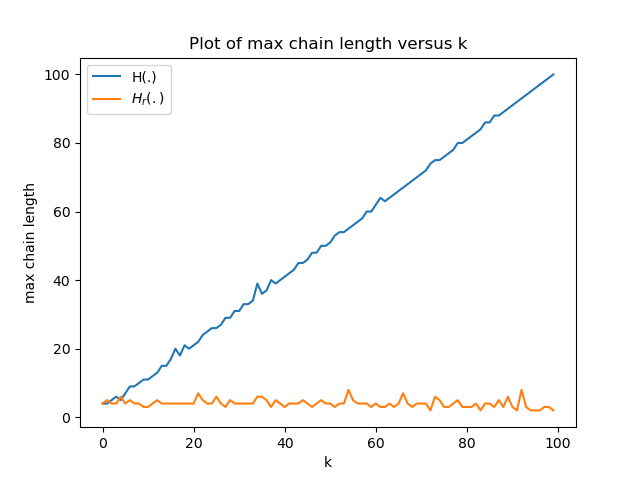
\includegraphics[width=0.5\linewidth]{4c.png}
        \caption{Plot}
      \end{figure}
      \inputminted{python}{4c.py}
    \end{proof}
\end{solution}

\end{document}
